\subsection{UDP / TCP}
To analyze the difference in power consumption between the two transmission methods,
we compared them. In the analysis, we paid attention to the elapsed time and power consumption during transmission. In the first comparison, 100 transmissions are compared.
\linebreak
\begin{table}[H]
    \begin{center}
    \caption{Comparison TCP UDP}
    \label{tab:table3}
    \begin{tabular}{|l|c|c|r|}
        \hline
        & \textbf{TCP} & \textbf{UDP} & \textbf{difference} \\
        & \multicolumn{2}{c|}{elapsed time [ms]} & \textbf{\%}\\
        \hline
        count & 100 & 100 & \\
        mean  & 241.57 & 95.97 & 39.73 \\
        std   & 32.115403 & 1.058444 & 3.30 \\
        min   & 193.0 & 94.0 & 48.70 \\
        25\%  & 219.0 & 95.0 & 43.38 \\
        50\%  & 236.0 & 96.0 & 40.68 \\
        75\%  & 257.0 & 97.0 & 37.74 \\
        max   & 396.0 & 98.0 & 24.75 \\
        \hline
    \end{tabular}
    \end{center}
\end{table}
\begin{figure}[H]
    \centering
    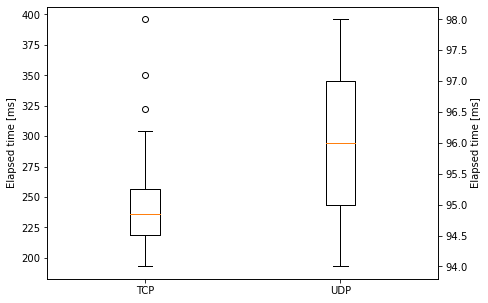
\includegraphics[width = 0.9 \linewidth]{fig/udp_tcp_elapsed_time_boxplot.png}
    \caption{Elapsed time when sending data over TCP and UDP}
    \label{fig:udp_tcp_boxplot_time}
    \end{figure}
If we compare the elapsed time spent sending the 1000 bytes,
we can save $96.0048 \pm 11.145 ms$ per cycle.
As shown in Table \ref{tab:table3},
we see that the range between the maximum and minimum send time for UDP is also much smaller.
As described in Chapter \ref{udp:sci}, UDP has less overhead while sending.
That's because it doesn't need energy to monitor sending cycle.
\begin{table}[H]
    \begin{center}
        \caption{Comparison TCP UDP}
        \label{tab:table4}
        \begin{tabular}{|l|c|c|r|}
            \hline
            & \textbf{TCP} & \textbf{{UDP}} & \textbf{difference} \\
            & \multicolumn{2}{c|}{ power consumption [As]} & \textbf{\%}\\
            \hline
            count & 100 & 100 & \\
            mean   & 0.021031 & 0.009227 & 43.87 \\
            std    & 0.002591 & 0.000581 & 22.42 \\
            min    & 0.0163 & 0.0082 & 50.31 \\
            25\%   & 0.019175 & 0.0088 & 45.89 \\
            50\%   & 0.0206 & 0.0091 & 44.17 \\
            75\%   & 0.022325 & 0.0096 & 43.00 \\
            max    & 0.0326 & 0.0109 & 33.44 \\
            \hline
        \end{tabular}
    \end{center}
\end{table}
\begin{figure}[H]
    \centering
    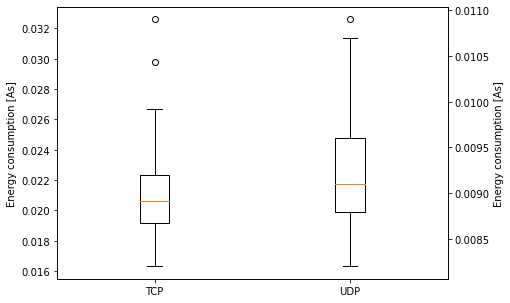
\includegraphics[width = 0.9 \linewidth]{fig/udp_tcp_power_consumption.png}
    \caption{Power connsumption when sending data over TCP and UDP}
    \label{fig:udp_tcp_boxplot_As}
    \end{figure}
In Table\ref{tab:table4} we compared the elapsed time while the ESP8266-01 sends.
As expected, we got the same result.
UDP requires only $44.03\% \pm 6.07\%$ of the time compared to TCP.
This gives us a saving of $0.00907018 \pm 0.00125 As$ while sending 1000 bytes.
For example, in Fig.\ref{fig:udp_tcp_s_m},
we compared the fiftieth cycle to see the differences between them.
In contrast, TCP requires much more power to establish the connection.
\begin{figure}[H]
    \centering
    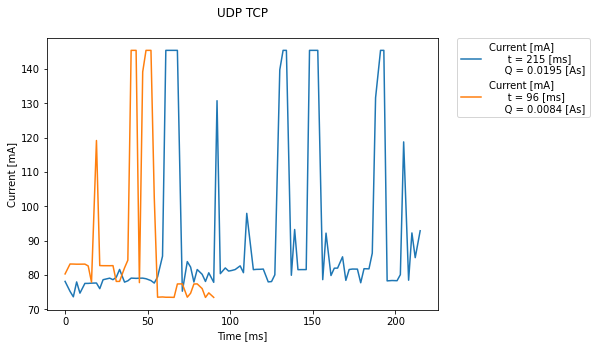
\includegraphics[width = 1 \linewidth]{fig/udp_tcp/udp_tcp_s_m.png}
    \caption{Sending data over TCP and UDP}
    \label{fig:udp_tcp_s_m}
    \end{figure}